\documentclass[conference]{IEEEtran}
\usepackage[utf8]{inputenc}
\usepackage[T1]{fontenc}
\usepackage[spanish,es-noshorthands]{babel}
\usepackage{graphicx,tabularx,array,xurl,placeins}
\renewcommand{\tabularxcolumn}[1]{>{\raggedright\arraybackslash}p{#1}}
\newcolumntype{P}[1]{>{\raggedright\arraybackslash}p{#1}}
\makeatletter\AtBeginDocument{\def\thesubsectiondis{\Alph{subsection}.}\def\@seccntformat#1{\csname the#1dis\endcsname\hskip 0.5em\relax}}\makeatother
\addto\captionsspanish{\renewcommand{\tablename}{TABLA}\renewcommand{\figurename}{Fig.}}
\renewcommand{\IEEEkeywordsname}{Palabras clave}
\begin{document}

\title{Alza la Voz: videojuego serio para que los testigos de acoso escolar aprendan a intervenir}

\author{

\IEEEauthorblockN{Felipe Raúl Ríos García}\IEEEauthorblockA{\textit{Gerencia}\\ \texttt{frrios@uninorte.edu.co}}\and \IEEEauthorblockN{Josue Salas Mercado}\IEEEauthorblockA{\textit{Código y diseño}\\ \texttt{josuems@uninorte.edu.co}}\and \IEEEauthorblockN{Gustavo Parody Cifuentes}\IEEEauthorblockA{\textit{Documentación}\\ \texttt{agparody@uninorte.edu.co}}\and \IEEEauthorblockN{Camilo Andrés Meriño Narváez}\IEEEauthorblockA{\textit{Pruebas}\\ \texttt{cmerinoa@uninorte.edu.co}}\and \IEEEauthorblockN{Avid Andrés Avila Rojano}\IEEEauthorblockA{\textit{UI/UX}\\ \texttt{avida@uninorte.edu.co}}

\and \IEEEauthorblockA{\textit{Nodo Sano Studios}\\ \textit{Estructura de Datos I (2026-30), profesor Ricardo Villanueva Polanco}\\ \textit{Universidad del Norte, Barranquilla, Colombia}}}

\maketitle

\begin{abstract}Cerca de uno de cada tres estudiantes dice haber sido acosado en el último mes, y en Colombia la proporción de estudiantes que reporta acoso está por encima del promedio de la OCDE. Casi siempre hay testigos, y la mayoría no hace nada. Alza la Voz es un videojuego de acción escrito en Python con pygame-ce para estudiantes de 10 a 15 años: el jugador protege a un compañero frenando los mensajes de acoso, deja llegar los de apoyo y, con cada acción valiente, convence a los testigos que solo miraban de que lo ayuden. El objetivo fue construir un juego que enseñe a intervenir por las consecuencias de cada acción, sin preguntas. Se compararon tres conceptos con cinco criterios, se definieron requerimientos con el modelo FURPS y se implementaron seis estructuras de datos propias (cola, pila, lista enlazada, lista circular, lista doble y multilista), además de archivos para las frases y los récords. La versión final tiene diez oleadas y un jefe final. En pruebas automáticas, un programa jugó partidas completas sin errores y el cálculo de cada cuadro tomó 1,4 ms. Cinco perfiles de bot probaron el juego y revelaron un fallo de balance que se corrigió.\end{abstract}

\begin{IEEEkeywords}juego serio, acoso escolar, testigos, estructuras de datos, Python, pygame\end{IEEEkeywords}

\section{Introducción}

Según la UNESCO, casi uno de cada tres estudiantes ha sido acosado por sus compañeros al menos una vez en el último mes \cite{ref1}. En Colombia, según PISA 2022, el 23 \% de las estudiantes y el 25 \% de los estudiantes reportaron sufrir actos de acoso al menos algunas veces al mes, frente al 20 \% y al 21 \% del promedio de la OCDE \cite{ref2}. Las redes sociales extienden el acoso fuera del colegio, porque los mismos comentarios llegan al celular por la noche. Usarlas de forma saludable incluye decidir qué hacer ante un comentario que hiere a otro: reírse, compartirlo, ignorarlo o frenarlo.

Quien acosa suele tener público, y lo que hace ese público influye en si la burla sigue o se detiene. Los testigos, sin embargo, tienden a no hacer nada. En un estudio con 194 estudiantes de séptimo y octavo grado, los que no jugaron el juego de la intervención consideraron con más frecuencia que el ciberacoso no era grave y que intervenir no les correspondía \cite{ref3}.

Existen videojuegos serios diseñados con este fin. Calvo-Morata et al. \cite{ref4} revisaron los que existen contra el acoso y el ciberacoso y concluyeron que ayudan a tomar conciencia del problema y a sentir empatía por la víctima, y que también pueden enseñar formas de responder. En un juego el jugador toma la decisión y ve el resultado de inmediato, algo difícil de lograr en una charla en el aula.

En Alza la Voz el jugador protege a Sam, un estudiante al que le llegan mensajes desde todos los bordes de la pantalla. Los de acoso hay que frenarlos; los de apoyo, dejarlos llegar. Es la misma decisión que enfrenta quien ve un comentario hiriente en un chat o en una red social. El jugador la repite muchas veces por partida, con el ratón y sin leer instrucciones largas, y cada diez puntos de valentía que gana, uno de los testigos que rodean a Sam se anima a ayudar. El objetivo del proyecto es desarrollar en Python un videojuego serio para estudiantes de 10 a 15 años que los entrene a intervenir cuando ven acoso, usando estructuras de datos implementadas por el equipo.

\section{Contribuciones}

La primera contribución es una mecánica de reacción rápida para enseñar a intervenir. En lugar de una historia que se lee, el jugador distingue en un segundo un mensaje de acoso (burbuja con picos) de uno de apoyo (burbuja redonda y verde) y actúa. Disparar a un apoyo tiene costo, así que la mecánica también entrena a no confundir una broma hiriente con un gesto amable.

La segunda es la representación del efecto contagio de la valentía. Ocho testigos rodean a Sam en gris; cada diez puntos de valentía, el siguiente del círculo se suma, se vuelve morado y empieza a defender a Sam. Esta idea se modeló con una lista circular, de modo que la estructura de datos y el mensaje del juego coinciden: el valor pasa de un vecino al siguiente.

La tercera es un juego completo con un código pensado para ser estudiado. La lógica y las estructuras caben en dos archivos de 812 y 244 líneas, comentados en español, y cada estructura se puede ver funcionando dentro del juego con un panel que se abre con la tecla F2. El arte (personajes, escenarios, burbujas e iconos) se dibuja por código, sin imágenes externas.

La cuarta es la validación del sistema con pruebas automáticas. Un programa juega partidas completas, prueba entradas erradas y archivos dañados, y cinco perfiles de bot juegan con teclado y ratón simulados; además, queda listo el protocolo para probarlo con personas.

\section{Trabajos relacionados}

Calvo-Morata et al. \cite{ref5} evaluaron Conectado, un juego en el que el jugador pasa varios días como estudiante nuevo y sufre acoso en el colegio y en las redes. Midieron la conciencia sobre el acoso antes y después de jugar y registraron lo que cada estudiante hizo dentro del juego. La conciencia aumentó en todos los grupos, y el aumento varió según las características y el comportamiento de cada jugador. En Conectado el jugador es la víctima; el papel del testigo queda fuera.

Ferreira et al. \cite{ref3} sí se enfocaron en los testigos. Su juego usa agentes sociales que reaccionan según el perfil del jugador, y busca que quien presencia ciberacoso defienda a la víctima. Repartieron al azar a 194 estudiantes en tres grupos: experimental (103), alternativo (37) y control (54). Según el análisis de covarianza, los que jugaron mostraron más conducta prosocial asertiva que el resto.

Achab Moukram et al. \cite{ref6} revisaron estudios que usaron recursos gamificados para prevenir el acoso escolar: de 606 trabajos encontrados en Scopus, PubMed, Web of Science y Dialnet seleccionaron 12. Según su revisión, las estrategias lúdicas sirven para identificar y trabajar variables asociadas al acoso, y usarlas en clase ayuda a crear conciencia y a prevenirlo. Como las intervenciones revisadas son muy distintas entre sí, la revisión no compara mecánicas concretas entre ellas.

Wei et al. \cite{ref7} midieron el efecto de rasgos concretos de diseño. Hicieron un juego narrativo sobre acoso escolar y dos estudios, con 130 y 250 participantes, en los que variaron cuánto se parecía el avatar al jugador y cuánto control tenía este dentro del juego. Los resultados fueron mixtos: solo cuando se jugaba desde el punto de vista de quien acosa el mayor control produjo la empatía buscada. En Alza la Voz el jugador no adopta esa perspectiva, pero el estudio muestra que el grado de control influye en la respuesta del jugador. Por eso el jugador actúa todo el tiempo.

Chen et al. \cite{ref8} probaron GISCC, que mezcla entrenamiento psicosocial con juegos de rol interactivos, en un ensayo aleatorizado con 105 adolescentes chinos: 55 en el grupo experimental y 50 en el de control. Compararon las mediciones de antes y después con ANCOVA y MANCOVA y encontraron una reducción significativa de las conductas de ciberacoso.

Özer y Bilgin \cite{ref9} evaluaron TheraBuddy, una novela visual web para promover que los testigos intervengan. Asignaron al azar a 138 estudiantes de 10 a 16 años de seis colegios de Ankara a un grupo de intervención (71) o a una lista de espera (67). Al mes, el puntaje de intervención activa subió más en el grupo que jugó, pero la interacción solo fue marginal (p = 0,08) y apenas el 43 \% había completado al menos el 10 \% del juego. Los autores lo interpretan como un efecto pequeño y temprano.

En estos trabajos los juegos tienen efecto, pero casi todos son narrativos o de rol, piden leer bastante y se aplican en sesiones guiadas. Ninguno de los trabajos revisados es un juego de reacción rápida en el que la lección salga de repetir una decisión de un segundo, y ese es el tipo de juego que se propone aquí. El dato de Özer y Bilgin sobre la poca gente que avanzó en su juego también pesó: Alza la Voz se entiende al verlo y una partida corta ya muestra la idea completa.

\section{Metodología}

\subsection{Alternativas de solución}

Se consideraron tres conceptos. En FEEDBACK el jugador maneja el teléfono de una adolescente durante un día; las publicaciones llegan en fila y para cada una tiene pocos segundos para disfrutarla, ignorarla, reportarla o guardarla como evidencia de acoso. Modo Avión pasa en una sola noche antes de un examen: el jugador usa un celular simulado, abre y cierra aplicaciones, intenta dormir a tiempo y de paso averigua quién maneja una cuenta anónima. Alza la Voz es de acción. Sam está en el centro, los mensajes llegan desde los bordes y el jugador dispara corazones a los de acoso sin tocar los de apoyo.

Cada concepto se calificó de 1 a 5 en cinco criterios (Tabla I). Los criterios se tomaron de las condiciones del proyecto: unas ocho semanas de trabajo y una evaluación en la Feria Gamer, donde cada jurado prueba el juego apenas unos minutos.

\begin{table}[!htbp]
\centering
\caption{Evaluación de alternativas (1 = peor, 5 = mejor)}
\footnotesize
\begin{tabularx}{\columnwidth}{|X|c|c|c|}
\hline
\textbf{Criterio} & \textbf{FEEDBACK} & \textbf{Modo Avión} & \textbf{Alza la Voz} \\ \hline
Facilidad de implementación & 4 & 2 & 4 \\ \hline
Tiempo de desarrollo & 4 & 2 & 5 \\ \hline
Comprensión en menos de un minuto & 4 & 3 & 5 \\ \hline
Uso natural de estructuras de datos & 5 & 5 & 4 \\ \hline
Riesgo técnico (5 = bajo) & 4 & 2 & 4 \\ \hline
\textbf{Total} & \textbf{21} & \textbf{14} & \textbf{22} \\ \hline
\end{tabularx}
\end{table}

Alza la Voz obtuvo el mayor puntaje total, con un punto de ventaja. FEEDBACK quedó cerca y en él las estructuras encajan muy bien, aunque obliga a leer cada publicación y eso hace lenta la primera partida. Modo Avión era el más inmersivo; simular la navegación de un celular, en cambio, costaba más tiempo del que había. En Alza la Voz bastaba con mirar la pantalla para saber qué hacer, porque los mensajes de acoso tienen picos y los de apoyo son redondos y verdes. También pesó que el grupo ya tenía una versión del juego en HTML y JavaScript, que se reescribió en Python.

\subsection{Requerimientos funcionales}

La Tabla II lista los requerimientos funcionales de la versión final. RF1 a RF7 describen la partida, RF8 y RF9 lo que se guarda y se consulta, y RF10 a RF12 la ayuda, la accesibilidad y el panel con el que se muestran las estructuras durante la sustentación.

\begin{table*}[!htbp]
\centering
\caption{Requerimientos funcionales}
\footnotesize
\begin{tabularx}{\textwidth}{|P{2.6cm}|X|}
\hline
\textbf{ID} & \textbf{Requerimiento} \\ \hline
RF1 & Mostrar a Sam en el centro y generar mensajes de acoso y de apoyo que avanzan hacia él desde ángulos aleatorios. \\ \hline
RF2 & Permitir que el jugador se mueva con W A S D o las flechas y lance corazones manteniendo el clic. \\ \hline
RF3 & Restar 12 de ánimo a Sam cuando lo alcanza un acoso y sumarle 6 cuando llega un apoyo. \\ \hline
RF4 & Cuando el jugador frena un apoyo, quitar 50 puntos, 8 de ánimo a Sam y parte del impulso, y decirle por qué. \\ \hline
RF5 & Llenar el impulso al frenar acoso y dejar llegar apoyo; con el impulso lleno, Espacio lanza una onda que frena el acoso a su alcance. \\ \hline
RF6 & Convertir un testigo en aliado cada 10 puntos de valentía; los aliados defienden lo que está cerca de Sam. \\ \hline
RF7 & Organizar la partida en diez oleadas, cada una con su escenario; la décima es un jefe con barra de vida. \\ \hline
RF8 & Guardar en un buzón cada apoyo que llega y permitir recorrerlo con las flechas en la pausa. \\ \hline
RF9 & Pedir el nombre al final y guardar los cinco mejores puntajes en un archivo. \\ \hline
RF10 & Ofrecer menú, pausa y una pantalla de ayuda desde el menú y durante la partida. \\ \hline
RF11 & Incluir un modo de alto contraste y subtítulos para los sonidos, salvo el del disparo, que se repite varias veces por segundo. \\ \hline
RF12 & Mostrar con F2 el estado de cada estructura de datos en tiempo real. \\ \hline
\end{tabularx}
\end{table*}

\subsection{Requerimientos no funcionales (FURPS)}

Para los requerimientos no funcionales se usó el modelo FURPS (Tabla III).

\begin{table*}[!htbp]
\centering
\caption{Requerimientos no funcionales según FURPS}
\footnotesize
\begin{tabularx}{\textwidth}{|P{2.6cm}|X|}
\hline
\textbf{Categoría} & \textbf{Requerimiento} \\ \hline
RNF1. Funcionalidad & El juego no hace preguntas explícitas: el jugador aprende por lo que pasa después de cada acción. Usa estructuras de datos propias, sin las listas de Python como pila o cola. \\ \hline
RNF2. Usabilidad & Un jugador nuevo sabe qué hacer en menos de un minuto. Los controles se ven en pantalla, cada acción tiene una respuesta visible y sonora, y hay avisos ante una tecla sin función. Lo motivan los puntos, los testigos que se suman y la pantalla de victoria. \\ \hline
RNF3. Confiabilidad & El juego no se cierra con teclas sin función, clics repetidos, nombres con caracteres raros ni archivos dañados o ausentes. Si falla un cuadro, vuelve al menú. \\ \hline
RNF4. Rendimiento & Corre a 60 cuadros por segundo con 40 mensajes en pantalla. \\ \hline
RNF5. Soporte & Las estructuras (estructuras.py) están separadas de la lógica (juego.py) y del dibujo (arte.py). Funciona en Windows con Python 3 y pygame-ce. \\ \hline
\end{tabularx}
\end{table*}

\subsection{Diseño de la solución}

La Fig. 1 muestra el diagrama de clases. Juego controla la partida y es dueño de las seis estructuras; Mensaje, Corazon y Testigo son los objetos que viven dentro de ellas. Las estructuras se construyen sobre Nodo, salvo la lista doble, que usa NodoDoble porque necesita la flecha al anterior. Las funciones de archivos leen las frases y guardan los récords, y el módulo arte entrega los dibujos ya hechos.

\begin{figure*}[!htbp]
\centering
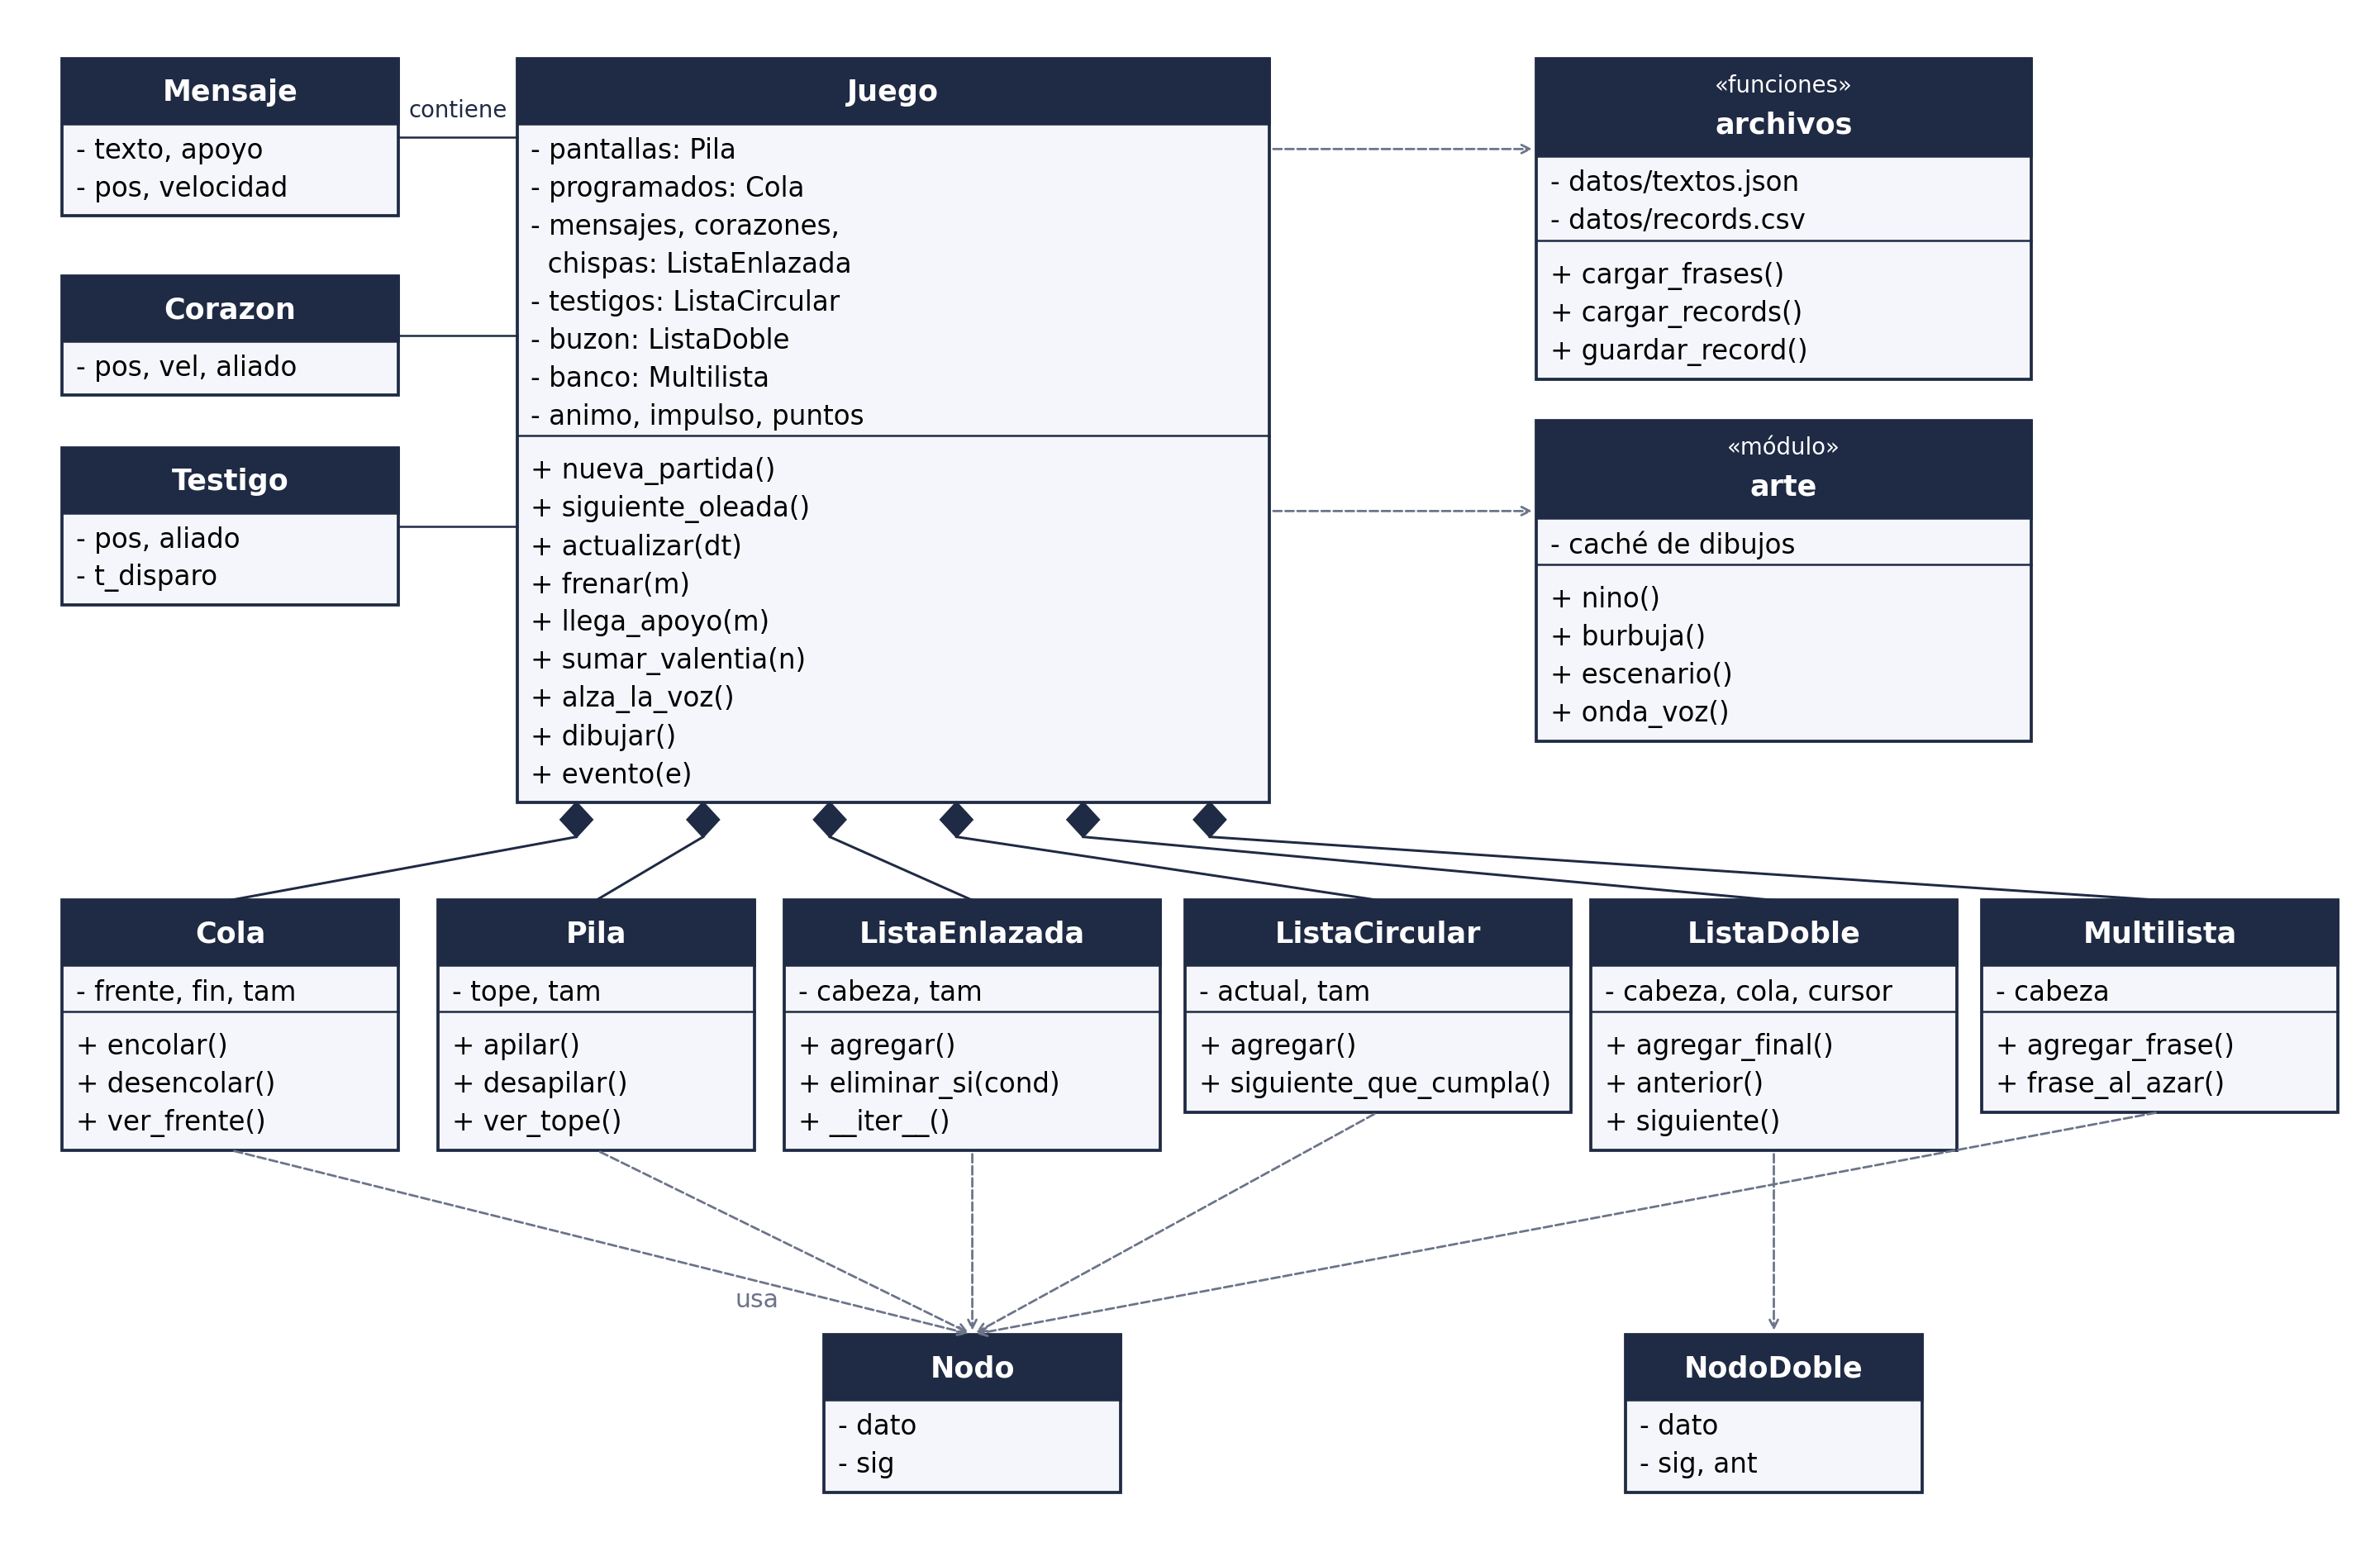
\includegraphics[width=0.9\textwidth]{figuras/diagrama_clases_final.png}
\caption{Diagrama de clases de la versión final.}
\end{figure*}

La Tabla IV resume para qué sirve cada estructura y por qué se eligió. El ciclo de un cuadro, en el método actualizar, sigue siempre el mismo orden. Primero los mensajes cuyo segundo ya llegó pasan de la cola a la lista enlazada; luego se mueven el jugador, los corazones y los mensajes, y se revisan los choques. Los mensajes que se frenan o llegan a Sam no se borran en ese momento: se marcan, y al final del cuadro eliminar\_si los quita de la lista en un solo recorrido. Así nunca se modifica una lista mientras se recorre.

\begin{table*}[!htbp]
\centering
\caption{Estructuras de datos y su uso en el juego}
\footnotesize
\begin{tabularx}{\textwidth}{|l|X|X|}
\hline
\textbf{Estructura} & \textbf{Uso} & \textbf{Por qué esta estructura} \\ \hline
Cola & Mensajes programados de la oleada (segundo, tipo y ángulo). & Salen en el orden en que se programaron (FIFO). \\ \hline
Pila & Pantallas abiertas: menú, juego, pausa, ayuda, récords y final. & Volver regresa a la última pantalla abierta (LIFO). \\ \hline
Lista enlazada & Mensajes, corazones, chispas y avisos en pantalla. & Se borran nodos de cualquier posición en un solo recorrido. \\ \hline
Lista circular & Los ocho testigos alrededor de Sam. & El valor pasa al siguiente vecino y, al llegar al último, el recorrido vuelve al primero. \\ \hline
Lista doble & Buzón con los apoyos que llegaron a Sam. & Se recorre hacia adelante y hacia atrás con las flechas. \\ \hline
Multilista & Banco de frases: 11 categorías, cada una con su lista (59 de acoso y 36 de apoyo). & Se busca la categoría y solo se recorre su sublista. \\ \hline
Archivos & textos.json (frases) y records.csv (cinco mejores puntajes). & Los datos se conservan al cerrar el programa y las frases se editan sin tocar el código. \\ \hline
\end{tabularx}
\end{table*}

\subsection{Entorno tecnológico}

El juego está escrito en Python 3 con pygame-ce 2.5, la versión de pygame que mantiene su comunidad \cite{ref10}. Python es el lenguaje que maneja todo el equipo, y en él las estructuras de datos se leen casi como pseudocódigo \cite{ref11}. pygame-ce resuelve la ventana, el dibujo, el sonido y la entrada de teclado y ratón, y se aprende más rápido que un motor completo. Los personajes, los diez escenarios, las burbujas y los iconos se dibujan con figuras simples a tres veces su tamaño y se reducen con suavizado; los sonidos se generan como ondas en el momento. Por eso el juego no depende de imágenes ni de audios externos. El código se escribió en Visual Studio Code y el informe en LaTeX con la plantilla de IEEE.

\subsection{Gestión del proyecto}

El equipo trabajó como la empresa Nodo Sano Studios. Felipe Ríos tuvo la gerencia; Josue Salas, el código y el diseño; Gustavo Parody, la documentación; Camilo Meriño, las pruebas, y Avid Avila, la interfaz y la experiencia de usuario. Se siguió un Scrum simplificado, con sprints de una semana que empezaban con una reunión corta. Las tareas se registraron en un tablero de Trello con las columnas Backlog, Esta semana, En proceso, En revisión y Hecho, y cada tarjeta llevaba responsable, etiqueta de rol y fecha límite.

\subsection{Evolución del prototipo}

En la primera entrega se presentó un prototipo de unas 370 líneas con tres oleadas y cuatro estructuras. Para la entrega final se llevaron a Python las mecánicas de la versión en JavaScript del grupo: el impulso y la onda de ``\textexclamdown{}Alza la voz!'', los testigos, el buzón, los escenarios y el jefe. Una primera versión completa llegó a unas 4.600 líneas, con cartas de mejora, varios tipos de enemigos y dos modos extra. Se decidió recortarla: cinco personas debían poder explicar todo el código en el examen individual, y esas piezas no cambiaban la idea central del juego. La versión final conserva las mecánicas que enseñan algo y deja juego.py y estructuras.py en 1.056 líneas; el dibujo, arte.py, ocupa otras 816. Quedaron por fuera el control con Arduino y la música de fondo.

\subsection{Uso de herramientas de inteligencia artificial}

Se usó Claude (Anthropic) para comparar conceptos de juego al comienzo, para generar y revisar código, para la capa de dibujo por código y como apoyo en la redacción de este informe. El equipo ejecutó y corrigió el código, decidió qué mecánicas quedaban en la versión final y buscó cada referencia en su fuente original. El aporte de la IA se estima en cerca de un 35 \%, concentrado en el arranque del proyecto y en la puesta en marcha de las ideas iniciales; en las etapas siguientes pasó a ser solo un apoyo.

\section{Resultados}

\subsection{Versión final del juego}

La Fig. 2 muestra el menú y la Fig. 3 una partida en la quinta oleada (Educación física): Sam en el centro, los testigos alrededor y las caras de los que ya ayudan en la parte superior. Cuando Sam pierde ánimo el escenario se vuelve azul y frío; cuando le llega un apoyo, Sam salta y su aura se enciende. La Fig. 4 muestra la onda de ``\textexclamdown{}Alza la voz!'' durante el jefe final y la Fig. 5 el modo de alto contraste, en el que el acoso y el apoyo se siguen distinguiendo por la forma.

\begin{figure}[!htbp]
\centering
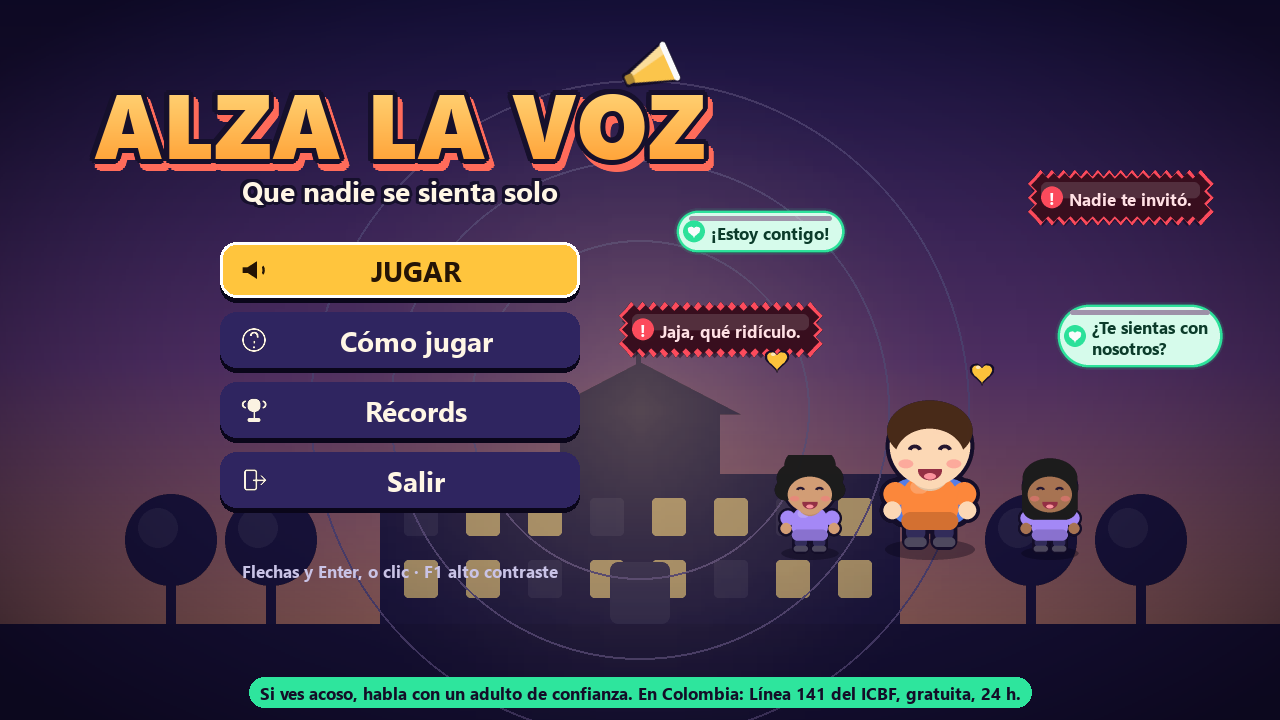
\includegraphics[width=\columnwidth]{figuras/01_menu.png}
\caption{Menú principal.}
\end{figure}

\begin{figure}[!htbp]
\centering
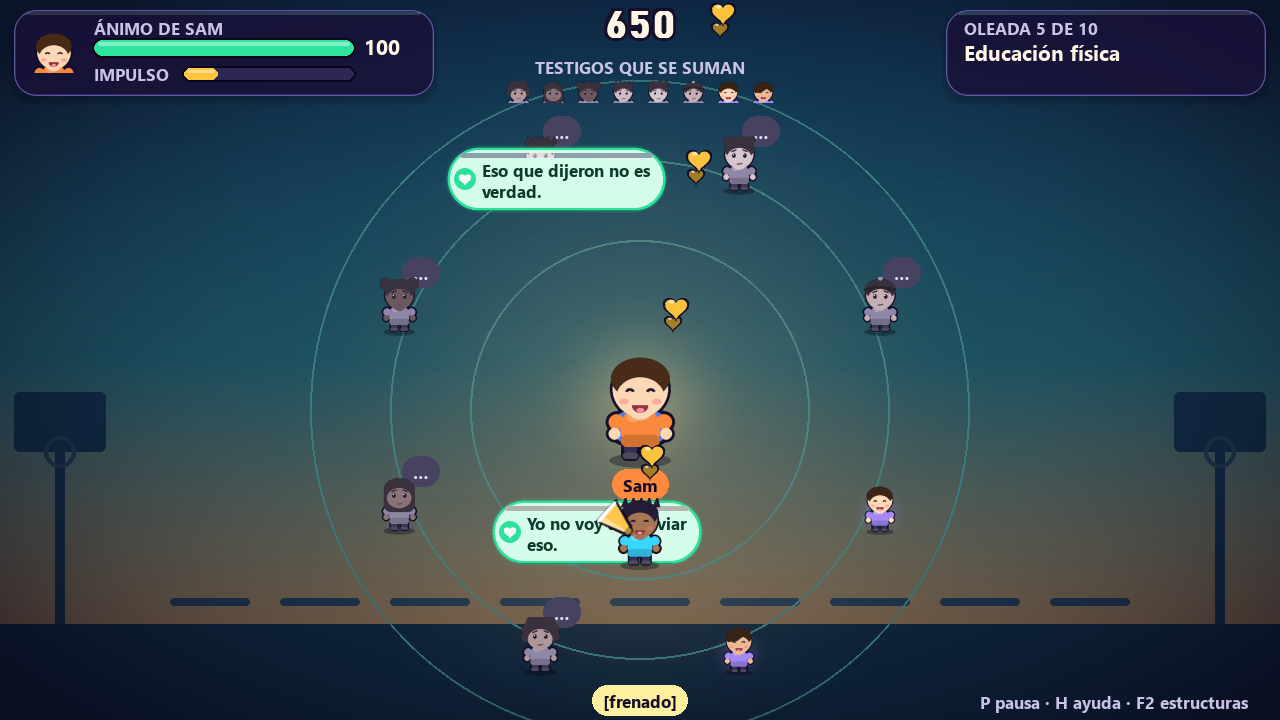
\includegraphics[width=\columnwidth]{figuras/03_oleada05.png}
\caption{Partida en la oleada 5: testigos grises que miran y morados que ayudan.}
\end{figure}

\begin{figure}[!htbp]
\centering
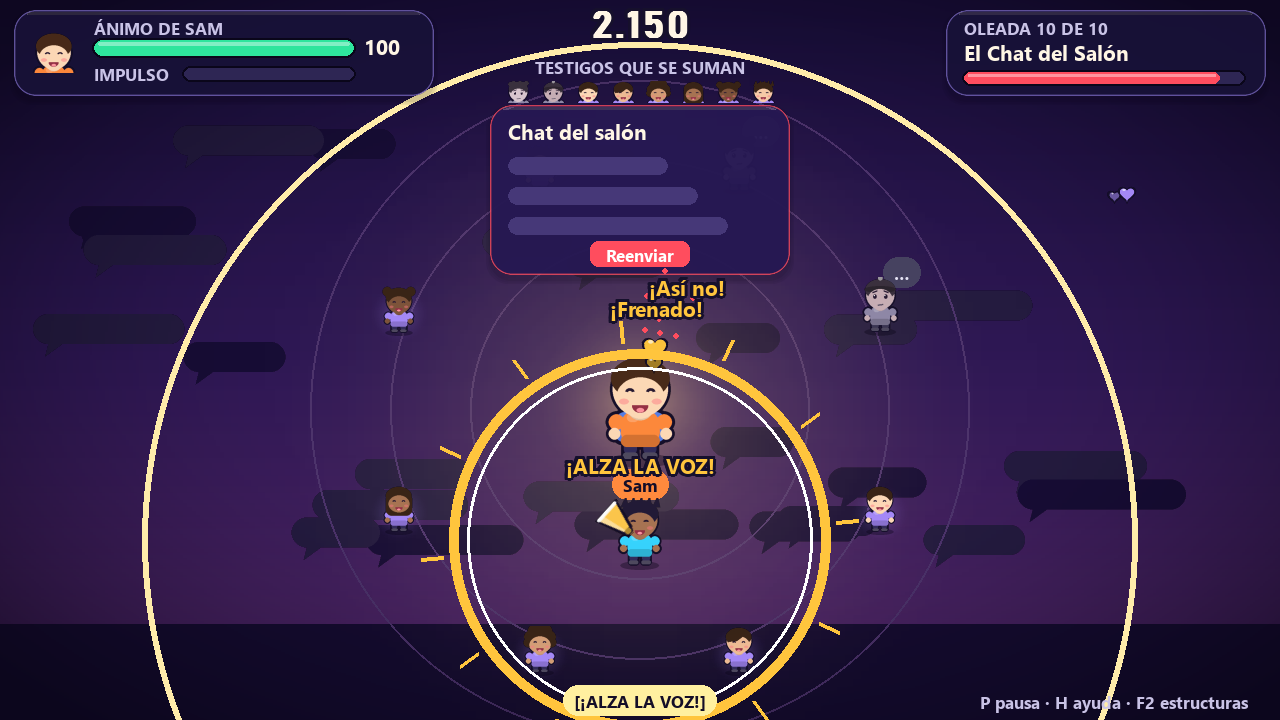
\includegraphics[width=\columnwidth]{figuras/04_alza_la_voz.png}
\caption{Onda de ``\textexclamdown{}Alza la voz!'' contra el jefe El Chat del Salón.}
\end{figure}

\begin{figure}[!htbp]
\centering
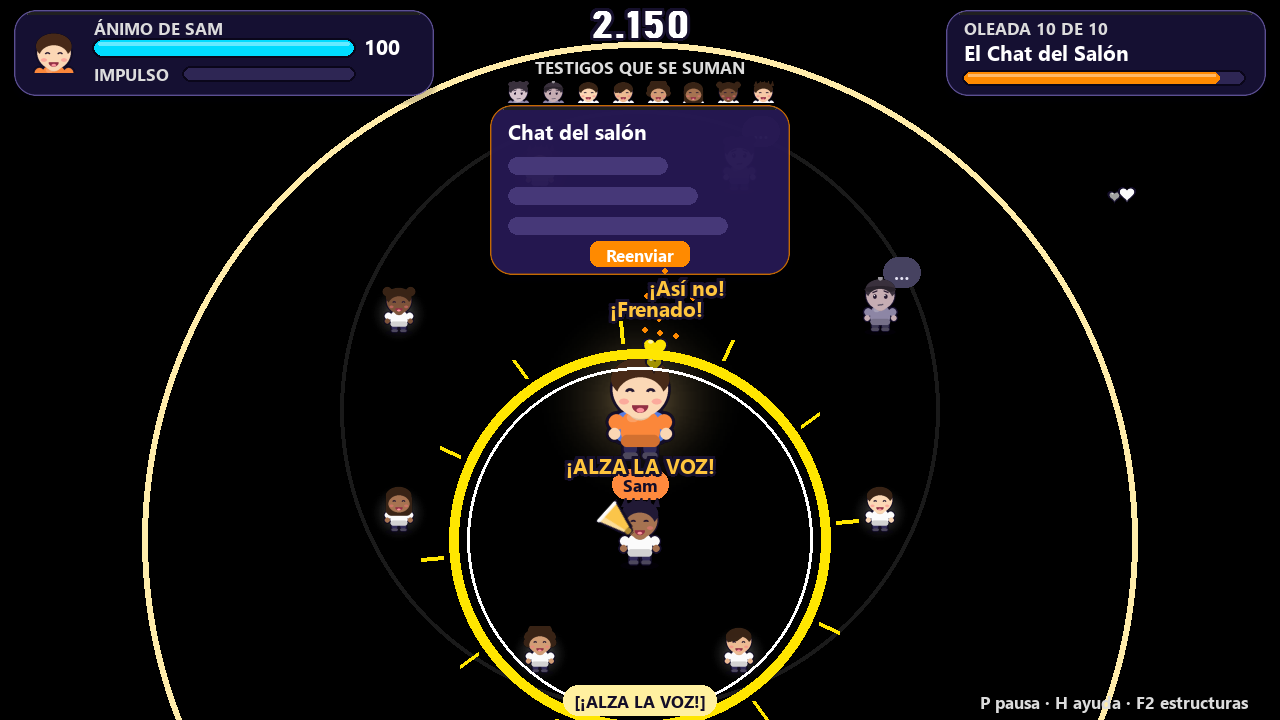
\includegraphics[width=\columnwidth]{figuras/06_alto_contraste.png}
\caption{Modo de alto contraste.}
\end{figure}

\subsection{Pruebas automáticas}

El script pruebas/test\_estructuras.py revisó cada estructura por separado: el orden de la cola y de la pila, el borrado en la lista enlazada al inicio, en medio y al final, la vuelta completa de la lista circular, los límites del cursor de la lista doble y la búsqueda por categoría en la multilista. Las seis pruebas pasaron. El script pruebas/simulacion.py jugó partidas completas sin intervención humana (Tabla V): en las tres primeras, el programa llegó a la décima oleada y venció al jefe.

\begin{table*}[!htbp]
\centering
\caption{Partidas automáticas}
\footnotesize
\begin{tabularx}{\textwidth}{|l|X|X|X|X|}
\hline
\textbf{Partida} & \textbf{Resultado} & \textbf{Frenados} & \textbf{Apoyos} & \textbf{Aliados} \\ \hline
Normal & Victoria (oleada 10) & 135 & 34 & 8 \\ \hline
Sam sin caer & Victoria (oleada 10) & 136 & 31 & 8 \\ \hline
Teclas al azar, Sam no cae & Victoria (oleada 10) & 143 & 26 & 8 \\ \hline
Quieto con 8 aliados (20 corridas) & Derrota, oleada 6 (5 a 8) & 44 & 32 & 8 \\ \hline
Quieto sin ayuda (20 corridas) & Derrota, oleada 2 (1 a 6) & 2 & 7 & - \\ \hline
\end{tabularx}
\end{table*}

Las dos últimas filas sirvieron para ajustar el balance. En una versión anterior los aliados disparaban cada 1,8 s a cualquier mensaje y el juego casi se jugaba solo. Ahora se suman cada 10 puntos de valentía y disparan cada 3,5 s, solo a lo que está a menos de 200 píxeles de Sam. Las dos últimas filas son medianas de 20 corridas con semillas distintas (pruebas/balance\_y\_rendimiento.py). Con los ocho aliados regalados y el jugador quieto, Sam cayó entre la quinta y la octava oleada, y en ninguna corrida hubo victoria.

La simulación también probó entradas erradas. Un nombre de prueba con símbolos, un emoji y 23 caracteres se guardó como ``Botñ 1234567'', y el juego arrancó y jugó con un archivo de récords dañado y sin el archivo de frases. En todas las corridas hubo cero errores. Con 40 mensajes y 150 chispas en pantalla, actualizar y dibujar un cuadro tomó 1,4 ms de mediana y 3,7 ms en el percentil 95, sin ventana; a 60 cuadros por segundo el límite es 16,7 ms.

\subsection{Prueba de usabilidad}

Para la prueba con personas se preparó un protocolo de prueba moderada según Moran \cite{ref12}: cada participante juega sin instrucciones previas mientras un integrante del equipo observa y toma notas, con cuatro tareas (entender qué hacer en el menú, frenar un acoso y dejar llegar un apoyo, usar ``\textexclamdown{}Alza la voz!'' y recorrer el buzón en la pausa), y al final responde la escala SUS \cite{ref13}, de diez preguntas con puntaje de 0 a 100. Esa prueba no se alcanzó a hacer antes de esta entrega, así que este informe no reporta datos de personas.

En su lugar se hizo una evaluación previa con pruebas/usabilidad\_bots.py, en la que cinco perfiles de bot jugaron usando solo el teclado y el ratón simulados, por el mismo camino que una persona (Tabla VI). En la primera corrida no hubo errores, pero los perfiles Novato y Gatillo fácil, que disparaban también a los apoyos, ganaron la partida, porque frenar un apoyo solo costaba 50 puntos. Con eso el juego no castigaba la confusión que busca enseñar. Se agregó que frenar un apoyo también le quita 8 de ánimo a Sam y 25 de impulso. La Tabla VI muestra la corrida después del cambio: los dos perfiles que no distinguen pierden en la tercera oleada y el que apunta solo al acoso sigue ganando. Los bots miden si el juego responde bien a cada tipo de jugador; si un estudiante entiende la regla en menos de un minuto (RNF2) queda por comprobar con personas.

\begin{table*}[!htbp]
\centering
\caption{Evaluación previa con cinco perfiles de bot}
\footnotesize
\begin{tabularx}{\textwidth}{|l|X|X|X|X|}
\hline
\textbf{Perfil} & \textbf{Cómo juega} & \textbf{Resultado} & \textbf{Primer acoso frenado} & \textbf{Disparos a apoyos} \\ \hline
Experto & Apunta solo al acoso y usa el impulso & Victoria (oleada 10) & 5,5 s & 26 \\ \hline
Novato & Apunta tarde y mal; abre la ayuda & Derrota (oleada 3) & 3,6 s & 14 \\ \hline
Gatillo fácil & Dispara a todo lo que se acerca & Derrota (oleada 3) & 5,6 s & 15 \\ \hline
Teclas al azar & Aporrea teclas, pausa, F1, F2 y Q & Reinicia en la oleada 1 & 5,0 s & 54 \\ \hline
Quieto & No toca nada & Derrota (oleada 1) & Nunca & 0 \\ \hline
\end{tabularx}
\end{table*}

\section{Conclusiones}

Alza la Voz cumplió los requerimientos funcionales y los no funcionales que se pudieron medir con pruebas automáticas; RNF2 depende de la prueba con usuarios. El juego tiene un componente aleatorio en el orden, el tipo y la dirección de los mensajes, y uno de habilidad en apuntar sin tocar los apoyos y en decidir cuándo usar el impulso. Para la accesibilidad tiene alto contraste y subtítulos. En ningún momento hace preguntas: la lección sale de lo que le pasa a Sam después de cada decisión. Las seis estructuras tienen un papel visible en la partida, y la lista circular de testigos representa la idea central del proyecto, que el valor se contagia.

Las pruebas automáticas mostraron un juego estable y con margen de rendimiento, pero no dicen nada sobre el aprendizaje. Un programa que gana todas las partidas no prueba que un estudiante vaya a intervenir cuando vea acoso en su colegio. La prueba con personas medirá si el juego se entiende; medir un cambio de conducta exigiría un estudio como los de Ferreira et al. \cite{ref3} o Özer y Bilgin \cite{ref9}, con grupos de control y seguimiento, que está fuera del alcance de este curso.

Hay otras limitaciones. El juego no tiene música de fondo, solo efectos de sonido, y no se construyó el control con Arduino previsto en la primera entrega. Las frases están en español y pensadas para Colombia. En una versión posterior se podrá medir con usuarios si el número de disparos a mensajes de apoyo baja entre la primera y la tercera partida, lo que indicaría que el jugador aprende a distinguir el acoso disfrazado de broma. También se podrá agregar un modo para el aula en el que el docente vea las frases que llegaron al buzón y las comente con el grupo.

\FloatBarrier

\begin{thebibliography}{10}
\bibitem{ref1} UNESCO, \textit{Behind the Numbers: Ending School Violence and Bullying}. París, Francia: UNESCO, 2019.
\bibitem{ref2} OECD, ``PISA 2022 Results (Volume I and II) -- Country Notes: Colombia,'' OECD Publishing, París, Francia, 2023. [En línea]. Disponible en: \url{https://www.oecd.org/en/publications/pisa-2022-results-volume-i-and-ii-country-notes_ed6fbcc5-en/colombia_dd5f34d9-en.html}. Consultado: 3 oct. 2026.
\bibitem{ref3} P. C. Ferreira, A. M. Veiga Simão, A. Paiva, C. Martinho, R. Prada y J. Rocha, ``Serious game-based psychosocial intervention to foster prosociality in cyberbullying bystanders,'' \textit{Psychosocial Intervention}, vol. 31, no. 2, pp. 83--96, 2022, doi: 10.5093/pi2022a5.
\bibitem{ref4} A. Calvo-Morata, C. Alonso-Fernández, M. Freire, I. Martínez-Ortiz y B. Fernández-Manjón, ``Serious games to prevent and detect bullying and cyberbullying: A systematic serious games and literature review,'' \textit{Computers \& Education}, vol. 157, 2020, Art. no. 103958, doi: 10.1016/j.compedu.2020.103958.
\bibitem{ref5} A. Calvo-Morata, C. Alonso-Fernández, M. Freire, I. Martínez-Ortiz y B. Fernández-Manjón, ``Creating awareness on bullying and cyberbullying among young people: Validating the effectiveness and design of the serious game Conectado,'' \textit{Telematics and Informatics}, vol. 60, 2021, Art. no. 101568, doi: 10.1016/j.tele.2021.101568.
\bibitem{ref6} Y. Achab Moukram, A. Manzano-León, J. M. Rodríguez-Ferrer, J. Rodríguez-Moreno y J. M. Aguilar-Parra, ``A systematic review of gamification as a playful strategy to prevent bullying,'' \textit{Environment and Social Psychology}, vol. 7, no. 2, 2023, doi: 10.18063/esp.v7.i2.1566.
\bibitem{ref7} L. Wei, M. Schmierbach, B. Liu, J. Kang, C. Chen, F. E. Dardis, R. Tan y O. Cohen, ``Amplifying player experience to facilitate prosocial outcomes in a narrative-based serious game,'' \textit{Media and Communication}, vol. 13, 2025, Art. no. 8637, doi: 10.17645/mac.8637.
\bibitem{ref8} Q. Chen, Z. Lu, B. Liu, Q. Xiao y K. L. Chan, ``Effectiveness of digital game-based GISCC program on cyberbullying prevention among Chinese adolescents,'' \textit{Child Abuse \& Neglect}, vol. 161, 2025, Art. no. 107293, doi: 10.1016/j.chiabu.2025.107293.
\bibitem{ref9} \.I. Ö. Özer y M. Bilgin, ``Enhancing active bystander intervention in bullying through a web-based visual novel: Preliminary findings from a randomized trial,'' \textit{International Journal of Bullying Prevention}, publicado en línea, 2026, doi: 10.1007/s42380-026-00353-5.
\bibitem{ref10} pygame-ce, ``Pygame Community Edition documentation.'' [En línea]. Disponible en: \url{https://pyga.me/docs/}. Consultado: 3 oct. 2026.
\bibitem{ref11} M. T. Goodrich, R. Tamassia y M. H. Goldwasser, \textit{Data Structures and Algorithms in Python}. Hoboken, NJ, EE. UU.: Wiley, 2013.
\bibitem{ref12} K. Moran, ``Usability testing 101,'' Nielsen Norman Group, 2019. [En línea]. Disponible en: \url{https://www.nngroup.com/articles/usability-testing-101/}. Consultado: 22 nov. 2026.
\bibitem{ref13} J. Brooke, ``SUS: A `quick and dirty' usability scale,'' en \textit{Usability Evaluation in Industry}, P. W. Jordan, B. Thomas, B. A. Weerdmeester e I. L. McClelland, Eds. Londres, Reino Unido: Taylor \& Francis, 1996, pp. 189--194.
\end{thebibliography}
\end{document}
